%Notes by Harsh Mistry 
%CS 341
%Based on Template From  https://www.cs.cmu.edu/~ggordon/10725-F12/template.tex

\documentclass[twoside]{article}
\setlength{\oddsidemargin}{0.25 in}
\setlength{\evensidemargin}{-0.25 in}
\setlength{\topmargin}{-0.6 in}
\setlength{\textwidth}{6.5 in}
\setlength{\textheight}{8.5 in}
\setlength{\headsep}{0.75 in}
\setlength{\parindent}{0 in}
\setlength{\parskip}{0.1 in}
\usepackage{amsmath,amsfonts,graphicx}
\newcounter{lecnum}
\renewcommand{\thepage}{\thelecnum-\arabic{page}}
\renewcommand{\thesection}{\thelecnum.\arabic{section}}
\renewcommand{\theequation}{\thelecnum.\arabic{equation}}
\renewcommand{\thefigure}{\thelecnum.\arabic{figure}}
\renewcommand{\thetable}{\thelecnum.\arabic{table}}
\newcommand{\lecture}[4]{
   \pagestyle{myheadings}
   \thispagestyle{plain}
   \newpage
   \setcounter{lecnum}{#1}
   \setcounter{page}{1}
   \graphicspath{ {images/} }
   
   
%Info Box 
   \begin{center}
   \framebox{
      \vbox{\vspace{2mm}
    \hbox to 6.28in { {\bf CS 341 -  Algorithms
	\hfill Winter 2018} }
       \vspace{4mm}
       \hbox to 6.28in { {\Large \hfill Lecture #1: #2  \hfill} }
       \vspace{2mm}
       \hbox to 6.28in { {\it Lecturer: #3 \hfill Notes By: #4} }
      \vspace{2mm}}
   }
   \end{center}
   
   \markboth{Lecture #1: #2}{Lecture #1: #2}



 
}

\renewcommand{\cite}[1]{[#1]}
\def\beginrefs{\begin{list}%
        {[\arabic{equation}]}{\usecounter{equation}
         \setlength{\leftmargin}{2.0truecm}\setlength{\labelsep}{0.4truecm}%
         \setlength{\labelwidth}{1.6truecm}}}
\def\endrefs{\end{list}}
\def\bibentry#1{\item[\hbox{[#1]}]}

\newcommand{\fig}[3]{
			\vspace{#2}
			\begin{center}
			Figure \thelecnum.#1:~#3
			\end{center}
	}

\newtheorem{theorem}{Theorem}[lecnum]
\newtheorem{lemma}[theorem]{Lemma}
\newtheorem{ex}[theorem]{Example}
\newtheorem{proposition}[theorem]{Proposition}
\newtheorem{claim}[theorem]{Claim}
\newtheorem{corollary}[theorem]{Corollary}
\newtheorem{definition}[theorem]{Definition}
\newenvironment{proof}{{\bf Proof:}}{\hfill\rule{2mm}{2mm}}
\newcommand\E{\mathbb{E}}


%Start of Document 
\begin{document}

\lecture{6}{January 23, 2018}{Bin Ma}{Harsh Mistry}
 \section{Divide and Conquer Continued}
 \begin{ex} Closest Pair\\
 \textbf{Input : } A set of points on plain: \(P= \{p_1, \ldots, p_n\}\) Each \(p_i = (x_i, y_i)\). Euclidean distance. \\
 \textbf{Output : } A pair of points \(p_1, p_j\) that are closest among all pairs\\
 
 
We use divide and conquer. The algorithm we are presenting needs the points to be sorted. Supposed P are sorted with x axis. Additionally, we have \(P^\prime\) containing references to all the  points and sorted according to y-axis. This requires \(O(\log m)\) time to sort the points. So we have \(P\), \(P^\prime\) to continue. 
 
For simplicity we assume all points have different x-axis for now.

First, we split \(P\) into two parts \(L\) and \(R\). With the assistance of \(I_x\), this can be done efficiently. 

\begin{center}
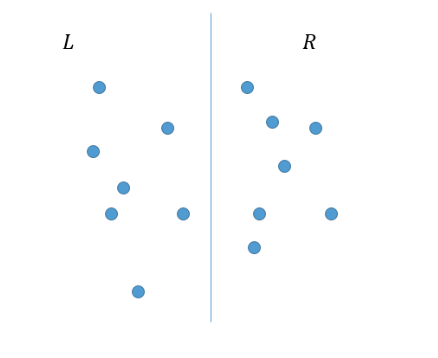
\includegraphics[scale=0.4]{4}
\end{center}
before we claim we can recursively solve the left and right parts, there is one more thing to do. Since we assume the bigger problem has \(P^\prime\) that are sorted according to y-axis, we need also ensure that the two smaller problems also have the y-axis sorted reference array. What we can do is to linearly scan through \(P^\prime\), and put the points into \(L^\prime\) and \(R^\prime\), depending on whether the point is at left or right of the split line. This takes \(O(n)\) time.


Now we can solve the left and right parts recursively. Let the least distance be \(\gamma_1\) and \(\gamma_2\). Let \(\gamma = min\{\gamma_1, \gamma_2\}\). The only remaining problem is the closest pair may be across the two parts nearby the split line. 

If \(l \in L \) and \(r \in R\) are such that \(d(l, r) \leq \gamma\), then they must be with in distance \(\gamma\) of the split line. So, we only need to limit our search within a narrow band around the split line as shown in the figure. We denote the list of points in this band by \(S\). Since \(P\) is sorted according to x-axis, \(S\) can be found in linear time. Additionally, we can linearly scan through \(P^\prime\) to construct an array \(S^\prime\) of references to points of \(S\), and make \(S^\prime\) sorted according to y-axis

Our goal is to find a pair (\(p, q\))from \(S\) within distance \(\gamma\). For each point \(p \in S\) with y-axis \(p, y\), we only need to compare it with the other points with y-axis between \(p, y\)and \(p.y + \gamma\) The above analysis indicates that there are at most 11 such points in \(S\). They are all clustered together in the y-axis sorted \(S^\prime\). The search takes 11⋅\(\mid S \mid \)=\(O(n)\) time. Let the minimum distance we find is \(\gamma_m\) Finally, we output \(min\{ \gamma, \gamma^\prime\}\) .If desired, the pair with the shortest distance can also be recorded during the above computation for output

\textbf{Time Complexity : } 
\[T(n) = 2 \cdot T(\frac{n}{2}) + O(n) \implies T(n) = O(n \log n )\] 

 \end{ex} 
 
\end{document}





